\documentclass{article}
\usepackage{graphicx}
\usepackage{tikz}
\usetikzlibrary{positioning, shapes.geometric, arrows.meta}

\title{Task 3.1: Deep FCNN on Tiny ImageNet Report}\date{February 3, 2026}

\begin{document}

\maketitle

\section{Introduction}
This report documents the implementation and analysis of a Deep Fully Connected Neural Network (FCNN) trained on a 10-class subset of the Tiny ImageNet dataset. The objective was to compare the training dynamics of Sigmoid activation versus Leaky ReLU with Batch Normalization in an 8-layer architecture.

\textbf{Hardware Specification:} The experiments were conducted on a single \textbf{NVIDIA RTX 4050 (6GB VRAM)}. The lightweight nature of the Deep FCNN allowed the entire batch and model to fit comfortably within the VRAM, ensuring efficient training.

\section{Architecture}
The network relies on \textbf{Circuit Theory} principles, utilizing depth to represent complex functions efficiently. It consists of an input layer (12,288 features) followed by 7 hidden layers.

\begin{figure}[h]
    \centering
    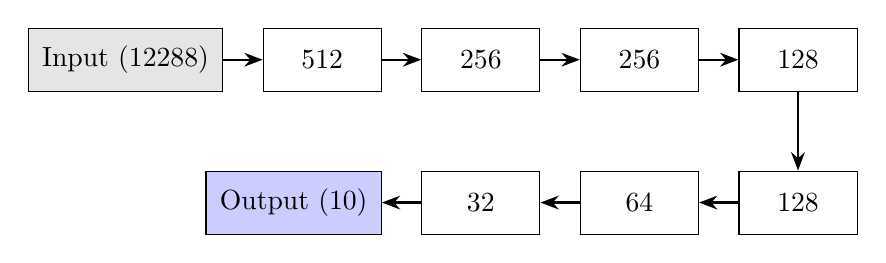
\begin{tikzpicture}[
        layer/.style={rectangle, draw=black, minimum width=1.5cm, minimum height=0.8cm, inner sep=5pt},
        arrow/.style={-Stealth, thick}
    ]
        \node[layer, fill=gray!20] (input) {Input (12288)};
        \node[layer, right=0.5cm of input] (h1) {512};
        \node[layer, right=0.5cm of h1] (h2) {256};
        \node[layer, right=0.5cm of h2] (h3) {256};
        \node[layer, right=0.5cm of h3] (h4) {128};
        
        % Break to next line for readability or continue if space permits. 
        % For compactness here, let's stack or continue.
        \node[layer, below=1cm of h4] (h5) {128};
        \node[layer, left=0.5cm of h5] (h6) {64};
        \node[layer, left=0.5cm of h6] (h7) {32};
        \node[layer, fill=blue!20, left=0.5cm of h7] (output) {Output (10)};

        \draw[arrow] (input) -- (h1);
        \draw[arrow] (h1) -- (h2);
        \draw[arrow] (h2) -- (h3);
        \draw[arrow] (h3) -- (h4);
        \draw[arrow] (h4) -- (h5); % Wrapping connection
        \draw[arrow] (h5) -- (h6);
        \draw[arrow] (h6) -- (h7);
        \draw[arrow] (h7) -- (output);
    \end{tikzpicture}
    \caption{Schematic of the 8-Layer Deep FCNN Architecture.}
    \label{fig:network}
\end{figure}

\section{Expectations}
Prior to experimentation, we established the following expectations:
\begin{itemize}
    \item \textbf{Vanishing Gradients:} We expect small gradient norms and the Vanishing Gradient Problem (VGP) in the Sigmoid network due to its depth.
    \item \textbf{ReLU + BN:} Learning should occur effectively with Leaky ReLU and Batch Normalization, as these mitigate VGP.
    \item \textbf{Overfitting:} As FCNNs are used on images (lacking spatial inductive bias), we expect overfitting in the absence of Dropout.
    \item \textbf{Complexity:} Simplifying the network architecture (reducing neurons per layer) might reduce overfitting.
    \item \textbf{Speed:} ReLU training speed is expected to be faster due to the elimination of computationally expensive exponential operations found in Sigmoid.
\end{itemize}

\section{Experiments}

\subsection{Experiment A: Sigmoid (No Batch Norm)}
\textbf{Configuration:} Activation function set to Sigmoid. No Batch Normalization applied.

\textbf{Observations:}
\begin{enumerate}
    \item \textbf{Vanishing Gradients:} The gradient norms in the first layer started extremely low ($0.0005$), confirming the vanishing gradient problem.
    \item \textbf{Performance:} The model underfitted significantly. Final Validation Accuracy reached only \textbf{26.2\%}, with training loss stalling around 1.6.
\end{enumerate}

\subsection{Experiment B: Leaky ReLU + Batch Normalization}
\textbf{Configuration:} Activation function set to Leaky ReLU ($\alpha=0.01$) with Batch Normalization.

\textbf{Observations:}
\begin{enumerate}
    \item \textbf{Healthy Gradient Flow:} Gradient norms remained stable ($>0.5$), enabling rapid learning.
    \item \textbf{Overfitting:} The model exhibited significant overfitting. Training loss dropped to \textbf{0.27}, while validation loss increased to \textbf{2.15}.
    \item \textbf{Performance:} Despite overfitting, the model achieved a peak validation accuracy of \textbf{40.4\%}.
    \item \textbf{Regularization:} We deliberately avoided Early Stopping as it is not an orthogonal method of regularization for this analysis.
\end{enumerate}

\section{Visual Evidence}
\begin{figure}[h]
    \centering
    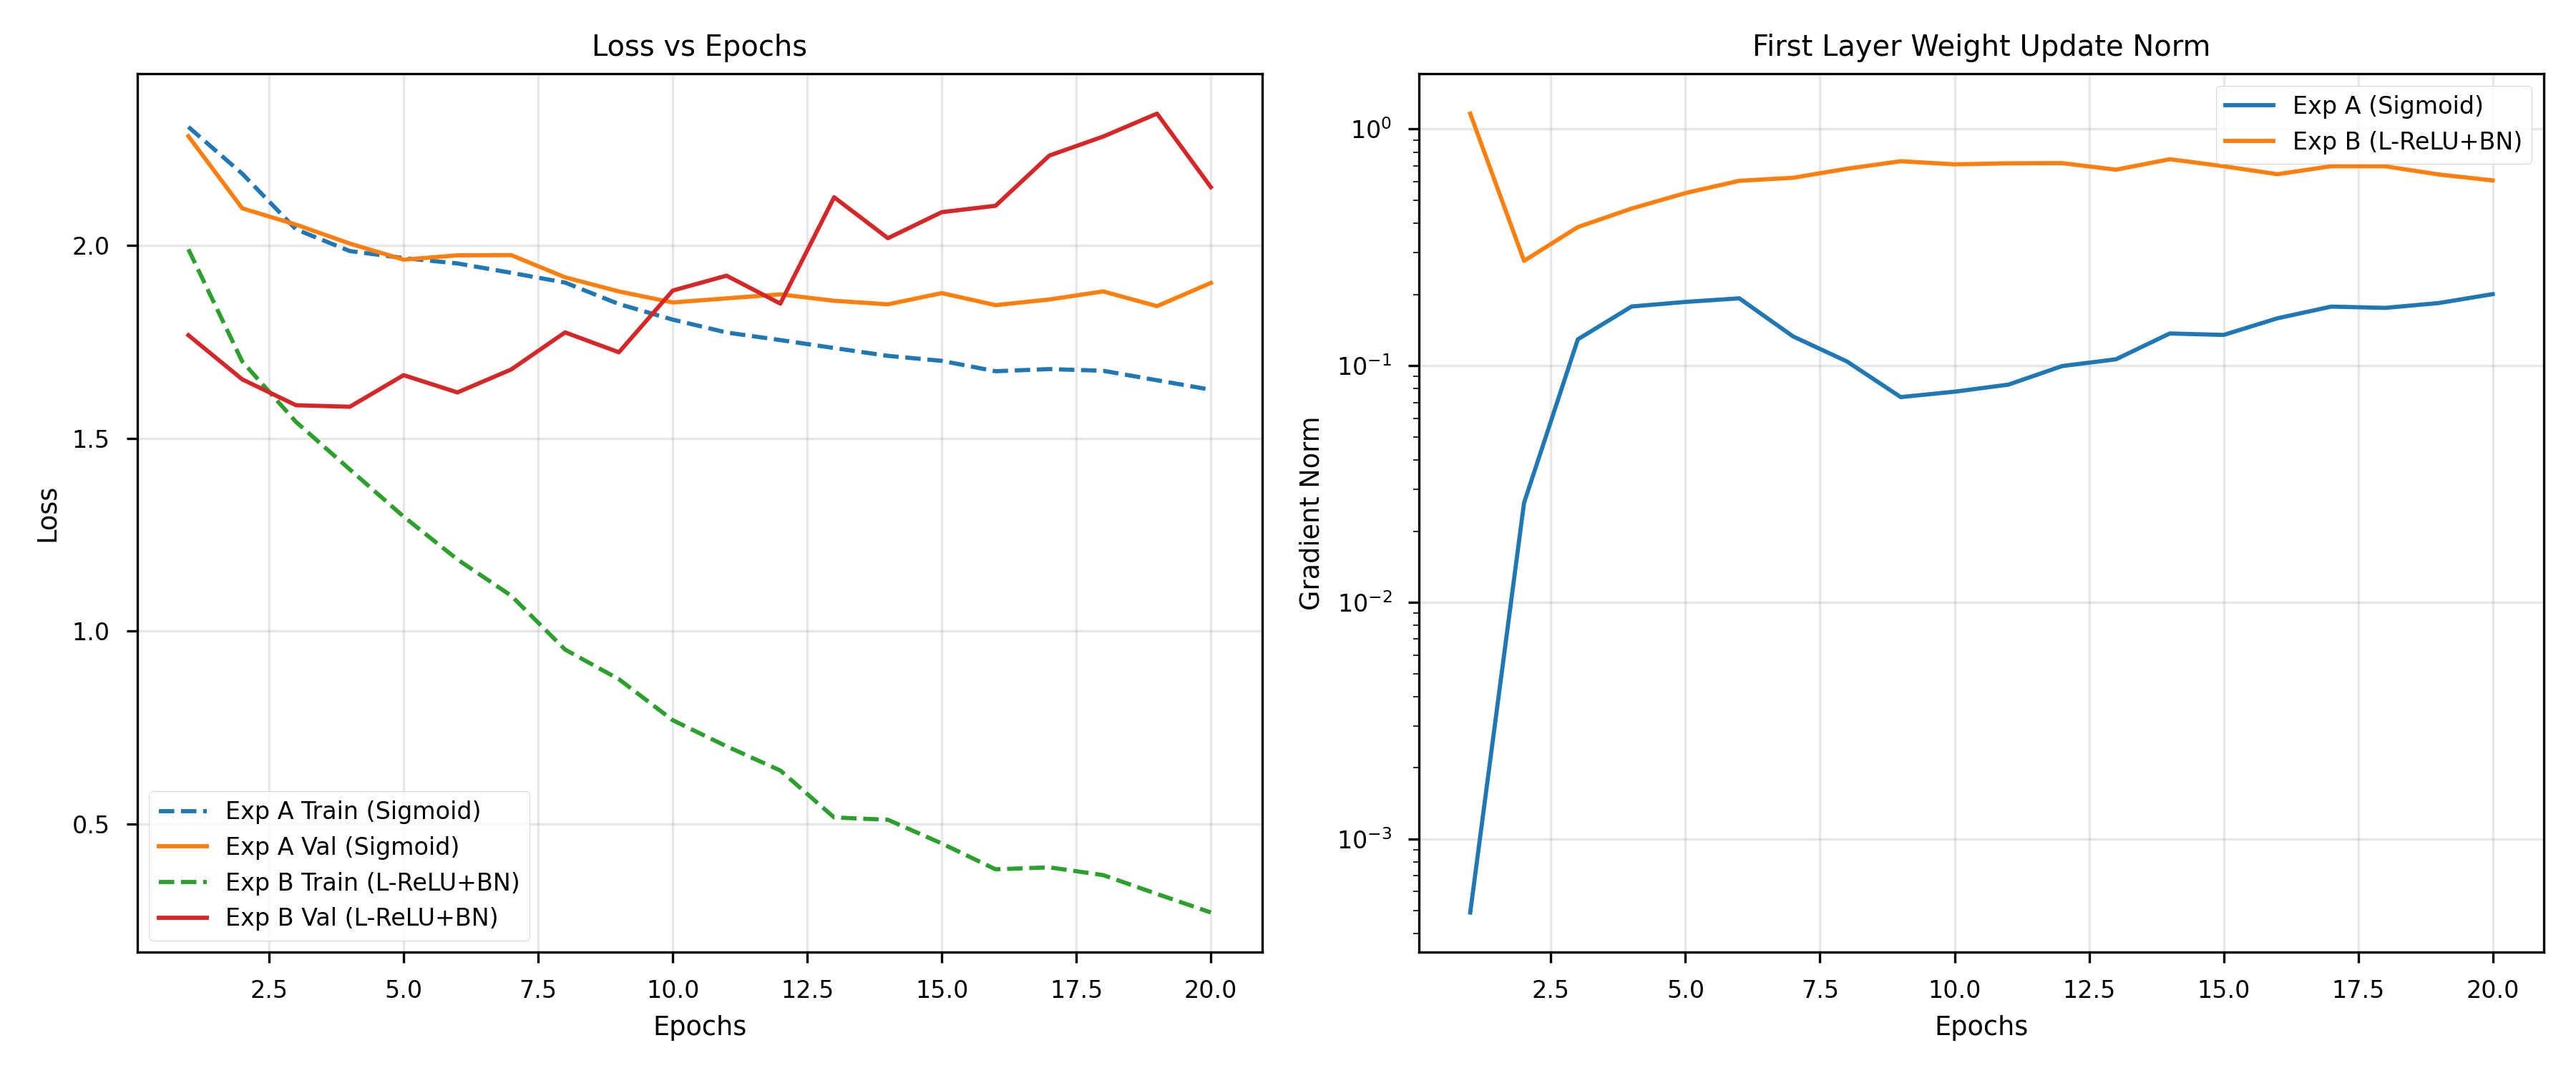
\includegraphics[width=1.0\textwidth]{plots/comparison_plot.png}
    \caption{Training Dynamics Comparison. Left: Loss vs Epochs showing Experiment B overfitting. Right: Gradient Norms showing Sigmoid (Experiment A) vanishing gradients.}
    \label{fig:results}
\end{figure}

\section{Conclusion}
The experiments demonstrate that \textbf{Leaky ReLU + BN} solves the vanishing gradient problem inherent in deep Sigmoid networks. However, the deep FCNN architecture is prone to overfitting on limited image data. 

\end{document}
